\documentclass[12pt]{article}
\usepackage[margin=1in]{geometry}
\usepackage[pdftex]{graphicx}
\usepackage{multirow}
\usepackage{setspace}
\usepackage{enumitem}
\pagestyle{plain}

\begin{document}

\noindent
% Course information
\begin{tabular*}{\textwidth}{l @{\extracolsep{\fill}} r}
  & \multirow{3}{*}{
\includegraphics[height=1.0in]{logo.jpg}} \\
  \large Particle Physics & \\
  \large Winter Quarter 2024 & \\
  \large Physics 130A & \\
\end{tabular*}
\vspace{10mm}

\noindent
% Professor information
\begin{tabular}{ l l }
  \multirow{6}{*}{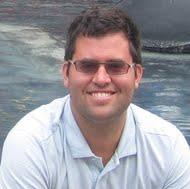
\includegraphics[height=1.25in]{mike.jpg}} & \\
  & \\
  & Michael Mulhearn \\
  & mulhearn@physics.ucdavis.edu \\
  & Physics 317 \\
  & \\
\end{tabular}
\vskip 0.5cm

\noindent
\begin{tabbing}
\hspace*{8em} \= \kill 
\textbf {Lecture:} \> M,W,F 9:00-9:50 AM in Roessler 148 
\end{tabbing}
\noindent
\begin{tabbing}
\hspace*{8em} \= \kill 
%\textbf{Textbooks:} \> Particle Physics (4th), Martin and Shaw.\\
\textbf{Textbooks:} \> Introduction to Elementary Particles (2nd), Griffiths.\\
\end{tabbing}
\noindent
\begin{tabbing}
\hspace*{8em}\= \hspace*{10em} \= \kill 
\textbf{Course TA:} \> (No Course TA)
\end{tabbing}
\noindent
\begin{tabbing}
\hspace*{8em}\= \hspace*{10em} \= \kill 
\textbf{Office Hours:}
    \> Mulhearn: \> Monday 10:00-11:00 AM PHY 317
\end{tabbing}
\noindent
\begin{tabbing}
\hspace*{12em}\= \kill 
\textbf{Homework:} \> From 5-10 homework problem sets.\\
\textbf{Quizzes:} \> From 5-10 homework quizzes.\\
\textbf{Midterm Exam:} \> TBD\\
\textbf{Final Exam:} \>  March, 21 2024 8:00 AM\\
\end{tabbing}
\noindent
\textbf {Course Description:}\\
Properties and classification of elementary particles and their interactions. Experimental techniques. Conservation laws and symmetries. Strong, electromagnetic, and weak interactions. Introduction to Feynman calculus.\\[3pt]

\noindent
\textbf{Homework:}\\ There will be 5-10 homework assignments.  They
will generally be due on Wednesday before lecture at 9 AM by
submission to gradescope.  You may consult with other students but
your submitted work must be your own.  Your homework will be graded on
effort only.\\[3pt]

\noindent
\textbf{Quizes:}\\
In the lecture following each homework assignment, you will usually take a short quiz.  The quizzes will be intended to test that you understood the homework you have submitted.  These quizzes should require no more preparation that looking over your own solutions.\\[3pt]

\noindent
\noindent
\textbf{Exams:}\\
Details on the midterm and final will be discussed later in the quarter.\\[3pt]

\noindent
\textbf {Grades:}\\
Final grades will be approximately $30\%$ homework, $30\%$ quizzes, $20\%$ midterm exam, 
and $20\%$ final exam. Your worst quiz score and worst homework will be dropped.  
You must also pass each component of the course (homework, quizzes, and both exams) in order to pass the course.  The passing level may be adjusted (lower than $60\%$) at my discretion. As this is the first time I have taught this course, I may adjust the relative weighting of each contribution to your final score, based on my observation of typical student outcomes.\\
\noindent


\noindent
\textbf {Course Schedule:}\\
This is a preliminary schedule which will evolve as the course progresses.\\

\noindent
\begin{tabular}{llll}
\textbf{Week} & \textbf{Dates} & \textbf{Topics} & \textbf{Reading} \\
\hline
1  & Jan 8,10,12      & Historical Introduction & 1.1-1.5    \\
\hline
2  & Jan 17,19        &                         &  1.6-1.11 \\
\hline
3  & Jan 22,24,26     & Elementary Particle Dynamics & 2.1-2.6 \\  
\hline
4  & Jan 29,31, Feb 2 & Relativistic Kinematics     & 3.1-3.5    \\
\hline
5  & Feb 5,7,9        & Feynman Calculus  & 6.1-6.3    \\
\hline
6  & Feb 12,14,16     & Quantum Electrodynamics & 7.1-7.9     \\
\hline
7  & Feb 21,23        & (Catch-Up)    & \\
\hline
8  & Feb 26,28, Mar 1 & Quantum Chromodynamics &   8.1-9.6\\
\hline
9  & Mar 4,6,8        & (Catch-Up)   & \\
\hline
10 & Mar 11,13,15     & Neutrino Oscillations (Time Permitting) & 11.1-11.5\\
\hline
\end{tabular}\\ \vskip 1cm


\end{document}

